\chapter{Data Acquisition}
\label{ch:sp-daq}

%%% todo

% Assign candidate names to sections and solicit them to write notes and/or presentations.

% Start and maintain a list holding links to all relevant notes and presentations.

\fixme{\textbf{Authors:}

  See \url{https://wiki.dunescience.org/wiki/Technical_Design_Report}
  for general guidance. 

  While this chapter is still in outline, \textbf{check that it hits all
  the required points} some of which are:

  We are to describe a \textbf{baseline} or \textbf{process to
  decide a baseline}.

  \textbf{BE SUCCINCT} $TDR \approx IDR + 10\%$, goal is 50 pages for
  this chapter. 

  You are encouraged to produce \textbf{tech notes} with any
  supporting verbosity which may be referenced.

  State requirements and demonstrate how they are met, use
  standardized requirements table.

  Emphasize safety and professionalism (projectisms: cost, schedule,
  risks, interfaces).}

\metainfo{Some sections of this chapter must be written generically
  and without any reference to module-specific terms. They are marked
  with an orange ``fixme'' box. 
  Yellow info boxes like this one provide guidance for the content. 
  This guidance is not comprehensive so authors may provide additional
  information but retaining \textbf{conciseness} and \textbf{not
    repeating} info in other section is required.}

\section{Introduction}
\label{sec:fd-daq:introduction}
\fixme{module-generic}

\metainfo{A brief introduction to this chapter describing what will be
  described.  This is \textbf{not} an overview of the DAQ itself.
  Keep it brief. Do \textbf{not} write a conceptual overview here,
  that is below, reference it. 
  Do \textbf{not} use module-specific language but \textbf{do}
  describe how commonalities are described in text shared by both
  SP/DP volumes and specialized sections appear only in their
  respective volume. 
  \textbf{Do} describe the lexicographical convention used to demark
  shared sections (this needs coordination with other chapters in the
  same boat).}

\section{Requirements}
\label{sec:fd-daq:requirements}
\fixme{module-generic}

\metainfo{One sentence introducing the contents of this section.}

\subsection{Specifications}
\label{sec:sd-daq:specifications}
\fixme{single-phase module}


\metainfo{Include rows of top-level requirements table (``Schmitz''
  table) here. 
  Augment that with any additional requirements of our determining. 
  Eg: accept data from detector electronics, perform reduction to
  satisfy output rate limit, allow for cross-module triggering,
  collect beam activity with XX\%, SNB requirements, noise level,
  total thermal and space envelop, etc....}

\metainfo{Include message passing requirements and domains.}

\subsection{Design Philosophy}

\metainfo{Describe how the design addresses the requirements.}

\subsection{Parameters}
\label{sec:sp-daq:parameters}
\fixme{single-phase module}

\metainfo{Include a table which lists all important parameters driving
  the design.  Sampling rate and resolution, channel count}


\section{Interfaces}
\label{sec:sp-daq:interfaces}
\metainfo{Include interface summary and table here.}
\subsection{TPC Cold Electronics}
\metainfo{Data reception physical and logical, configuration information delivery.}
\subsection{PDS Readout System}
\metainfo{Data reception physical and logical, configuration information delivery.}
\subsection{Computing}
\metainfo{Buffer disk. 
  Agreement on sysadmin support and computer procurement, ssh gateways, non data networks. 
  Address reference how the data model described above is acceptable.}
\subsection{CISC}
\subsection{Calibration}
\subsection{Timing}
\metainfo{Note, this is an ``outgoing'' interface from DAQ's Timing System to various others. 
  Instead of making this section explicit we may instead disperse Timing System interface information among the other Interface sections where appropriate.}

\section{ProtoDUNE and DUNE Comparison}

\metainfo{Here we write what similarities and differences there are between ProtoDUNE and DUNE DAQ designs.}

\subsection{Detector Readout Hardware}

\metainfo{Compare and contrast design elements related to the detector readout hardware.}

\subsubsection{RCE}

\subsubsection{FELIX}

\subsection{Backend Event Building}

\subsection{Other}

\section{DAQ Design}
\label{sec:fd-daq:design}
\fixme{module-generic}

\metainfo{One sentence to introduce the section. 
  Listing the subsections and describing which are generic and which
  are X-phase specific.}

\subsection{Overview}
\label{sec:fd-daq:design-overview}
\fixme{module-generic}

\begin{dunefigure}{fig:daq-conceptual-overview}{DAQ Conceptual
    Subsystem Overview. 
    Concrete hardware or software systems may span multiple subsystems
    or cover only portions of a subsystem. High level walk through of
    and referencing the remaining subsections in this section. }
  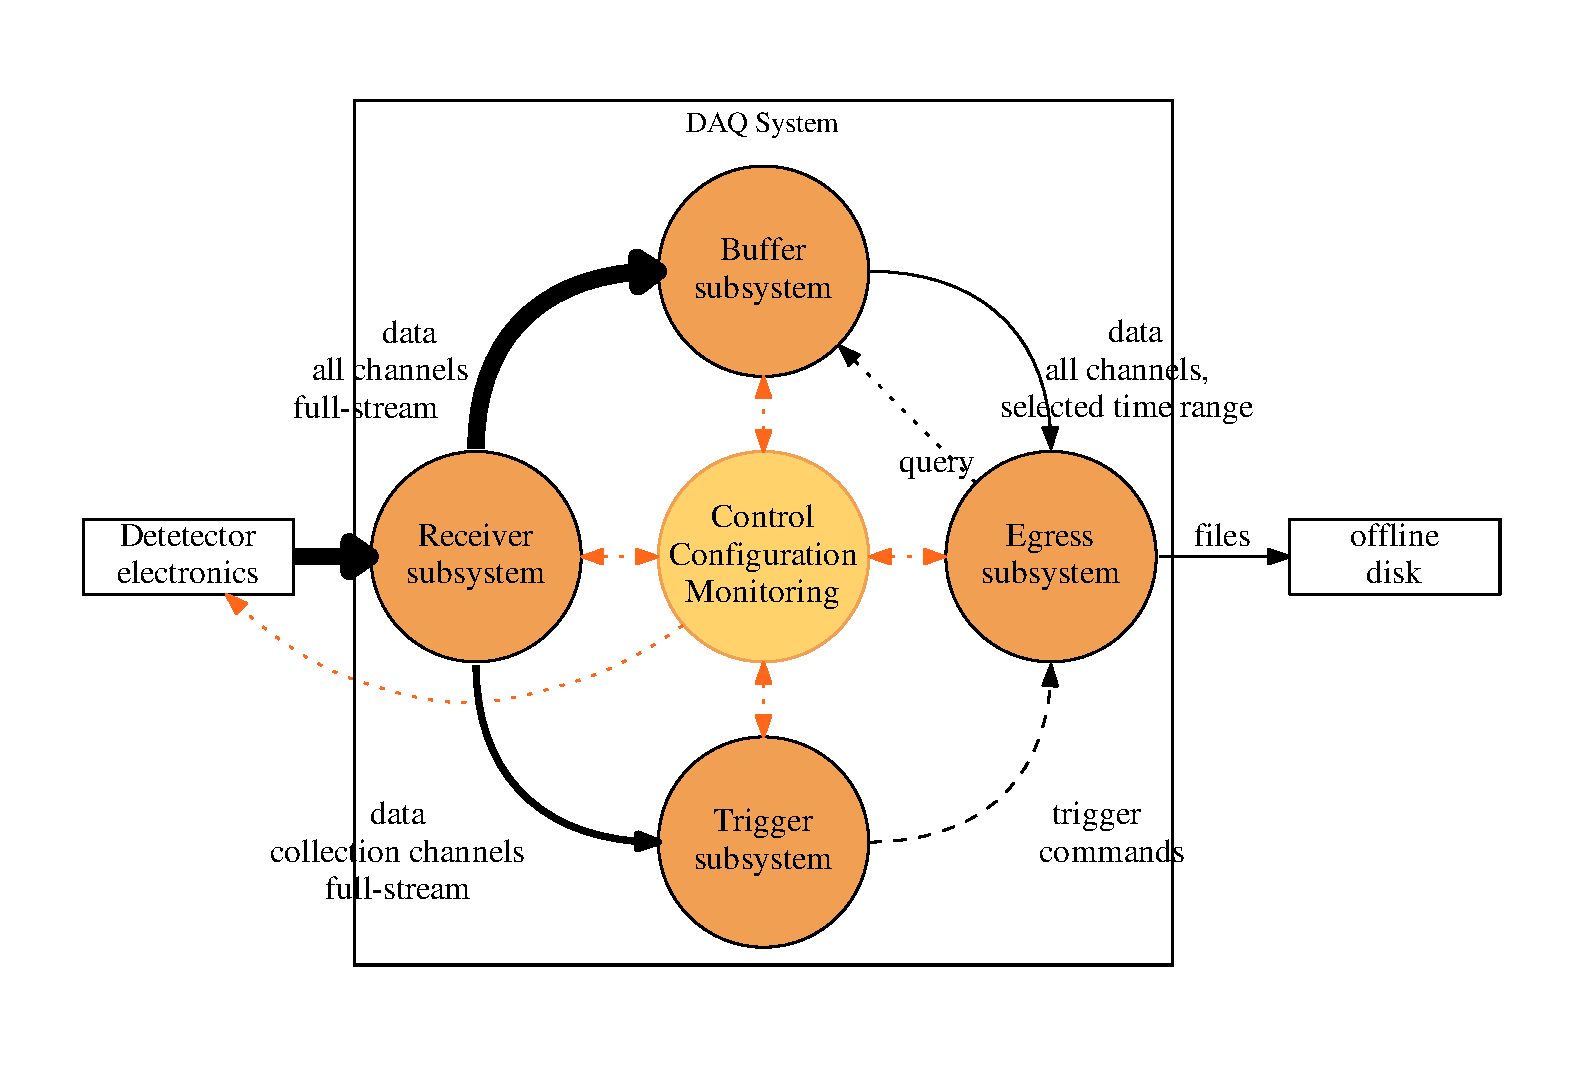
\includegraphics[width=0.8\textwidth]{daq-toplevel-conceptual.pdf}
\end{dunefigure}

\metainfo{This is the \textbf{only} place to describe the conceptual
  overview. 
  Do \textbf{not} repeat this info in sections below. 
  \textbf{Do} use \textbf{module-neutral} terms.
  \textbf{Do} describe major interface between each subsystem (the edges between the circles in Fig~\ref{fig:daq-conceptual-overview}).
  \textbf{Do} mention that concrete systems span portions of the
  conceptual subsystems and how the following subsections are defined
  along these concrete deliverable lines.}

\metainfo{Include components summary and table here.}

\metainfo{Include physical location description}

\metainfo{For the following sections, do not include directly validation info but rather place this information in section~\ref{sec:sp-daq:design-validation} and make references.}
  



\subsection{Message Passing}
\label{sec:fd-daq:design-messages}
\fixme{module-generic}

\metainfo{Describe the domains requiring message passing.  A domain means parts that shall share the same message passing infrastructure.  Eg, the hierarchical trigger system is one.  The transfer of data between artDAQ nodes is another.  Run control, monitoring and logging is a third.  Some MP domains will exist in other consortia and must interface with DAQ MP domains.  Each internal or external interface must be at least listed.   Describe how effort will be conserved by minimizing the number of distinct domains to the extent it makes sense.  Some examples: two-way comms with CISC (CISC tells DAQ of HV it shut down, DAQ tells CISC about hardware health, DAQ process health, statistics on things like per-unit trigger rates), handling laser triggers (eg, want laser to only fire in between beam spills).}

\metainfo{We may not be ready to give concrete designs for every domain.  Where this is the case, we must describe a plan for determining the MP system for each domain.}

\metainfo{Message passing must support redundant paths for trigger information, especially at the MLT level and above, to assure robustness.}


\subsection{Run Control and Monitoring}
\label{sec:fd-daq:design-run-control}
\fixme{module-generic}

\metainfo{Describe run control and DAQ operation monitoring. 
  How it makes use of the Message Passing System. 
  What is an ``epoch''.
  How Epoch Change Requests lead to zero down time reconfiguration. 
  Public key based ``iron'' authentication between run control processes and the controlled processes. 
  Describe how RC will configure partitioning, initiate reconfiguration, handle ``run'' changes, node discovery, configuration, logging, startup, shutdown and failures are handled. Describe how RC will support detector electronics configuration.}

\subsection{Front-end Data Handling and Processing}
\label{sec:sp-daq:design-fe-processing}

\metainfo{This section describes four functional blocks: (1) 10s RAM buffer (minimum), (2) non-volatile SNB buffer for 30s of data once per month (minimum), (3) hardware for the production of trigger primitive including any data formatting and DPS filtering and (4) compression of selected data.  Note, actual algorithms for trigger primitives are described in Section~\ref{sec:sp-daq:design-selection-algs}.}

\metainfo{One or two sentences that positions the two processing
  patterns (FEDHP either before or after FELIX) in this section as options. 
  Say that the ``FPGA before FELIX'' option is used for ``baseline costing''.}

\metainfo{Include a table with one row for each known compression factor: protoDUNE RCE and FELIX, MicroBooNE before and after noise filter (see docdb), 35t, protoDUNE data after ADC stuck code mitigation or avoidance, simulations.  One column of this table shall give a brief comment of how it applies to DUNE including any caveats or reasons for over/under estimation.}

% \subsubsection{FELIX+FPGA}
\subsubsection{Upstream FPGA and Firmware}
\label{sec:sp-daq:design-felix-fpga}
\fixme{single-phase module}

\metainfo{Include full hardware scope starting at fibers from CE and
  ending at the output of trigger processors and the interface between
  buffer and the Data Selector.
  Describe the per-APA multiplicity of computers, CPU cores, host
  system RAM, host system storage, FELIX boards, DPM components (RAM,
  SSD). 
  Include thermal estimates itemized by components.}

% \subsubsection{FELIX+CPU}
\subsubsection{Downstream CPU and Software}
\label{sec:sp-daq:design-felix-cpu}
\fixme{single-phase module}

\metainfo{Include full hardware scope starting at fibers from CE and
  ending at the output of trigger processors and the interface between
  buffer and the Data Selector. 
  Describe the per-APA multiplicity of computers, CPU cores, host
  system RAM, SSD and FELIX boards. 
  Include thermal estimates itemized by components.}


\subsubsection{Photon Detection System Interface}

\metainfo{Some motivations for using light to trigger. 
  (1) want to understand PDS so want to trigger on just the PDS. 
  (2) background to SNB for which PDS trigger primitives may eliminate. 
  (3) possibly must rely on light only for SNB triggering, eg if noise is out of control. 
  Some to all of these should be included.}

\metainfo{Possibly want to \SI{1}{\micro\second} packet for every time a 1-PE threshold is crossed. 
  PDS is still understanding what they may send. 
  DAQ needs to be in control of the trigger forming.}

\subsubsection{DP TPC FE issues}

\fixme{dual-phase module}

\metainfo{This is similar to SP except for the need to decompress before any trigger primitive processing.  Decompression can potentially happen on FELIX FPGA or on CPU.  There shall be a table or description of the amount of processing required.}

\subsubsection{DP SP Issues}
\fixme{dual-phase module}




\subsection{FELIX Hardware}
\label{sec:fd-daq:design-felix}
\fixme{module-generic}

\metainfo{Describe how FELIX hardware defines an interface which common to all modules.  Describe how the hardware may handle UDP or other prototocols including bidirectional communication.  Describe how FELIX can be scaled to accept data across a spectrum in order from large to small data rate: the full SP data from the WIBs, full compressed data from the DP, trigger primitive stream from FPGA based units placed between WIBs and FELIX.}


\subsubsection{DP data ingest via UDP}
\label{sec:dp-daq:design-udp-ingest}
\fixme{dual-phase module, move to DP-DAQ chapter eventually}
\metainfo{This is a DP section and will be only in the DP volume. 
  It should describe the ``Bump On Wire'' from the IDR unless we can
  come up with any new/better ideas.}
\metainfo{Include full hardware scope starting at fibers from CE and
  ending at the output of trigger processors and the interface between
  buffer and the Data Selector.
  Describe the per-APA multiplicity of computers, CPU cores, host
  system RAM, host system storage, FELIX boards, DPM components (RAM,
  SSD). 
  Include thermal estimates itemized by components.}  


\subsection{Data Selection}
\label{sec:sp-daq:design-selection-algs}
\fixme{single-phase module}

\fixme{There are many studies which could go into this section. Some of this may very likely be moved into one or more tech notes and referenced.}


Data Selection must make the decision about what data will be
transferred to the Backend Subsystem. 
It does by providing the core payload software which runs in message
passing nodes. 
In particular it provides the trigger primitive, candidate and
command hierarchy.

\metainfo{One sentence that briefly describes the ``bow tie''
  hierarchy: primitive, candidate, command, query. 
  Do not repeat too much what is in the design overview. 
}


\subsubsection{Trigger Primitives}
\label{sec:sp-daq:design-trigger-primitives}
\fixme{single-phase module}

\fixme{Trigger primitive algorithms run inside of the hardware of \ref{sec:sp-daq:design-fe-processing} but conceptually are more intimate with the Data Selection.  That section should reference this section.}

\metainfo{Describe what they are, how they are formed, storage size on disk, message schema. 
  This section describes algorithms with references to where those algorithms may run (FPGA firmware or CPU software)} \metainfo{Reference the section that provides validation.}


\metainfo{Include plot and discussion of DUNE trigger primitive rate in protoDUNE. 
  The fact that this includes many more cosmics will not matter much as the rate is expected to be dominated by Ar39. 
  Phil has this already but the LAr purity is not yet high enough to see Ar39 across the whole drift distance.}

\subsection{Backend System}
\label{sec:fd-daq:design-backend}
\fixme{module-generic}

\metainfo{This subsystem starts with receiving trigger commands from MTL, based on their content it queries Data Selectors on all front end computers, forms events, writes files to offline buffer disk. 
  It may perform ``offline'' type processing along the way.}


\subsubsection{Event builder}
\label{sec:fd-daq:design-event-builder}
\fixme{module-generic}

\metainfo{Explain artDAQ, handling of trigger commands by asynchronous, parallel queries to front end Data Selector (but take care not to duplicate between here and in the overview).}

\subsubsection{L2 Data Reduction}

\subsubsection{Data Quality Monitoring}

\subsubsection{Data Model}
\label{sec:fd-daq:design-data-model}
\fixme{module-generic}

\metainfo{Describe the data model. 
  This isn't a strict schema just things like how various parts of the
  detector readout map to files, etc.}

\subsubsection{Output Buffer}

\metainfo{Describe the output buffer system, how it's shared with offline, data hand-off prototocols.  Responsibility scope (eg, who handles transfer to FNAL).}

\subsection{Timing Distribution}
\label{sec:sp-daq:design-timing}
\fixme{single-phase module}
\fixme{Is it indeed still single-phase specific?}

\metainfo{Hardware, consumers, links.}

\subsection{Design Validation and Development Plan}
\label{sec:sp-daq:design-validation}
\fixme{single-phase module}

\metainfo{One sentence to describe our validation strategy: exploit
  ProtoDUNE, use simulation and develope vertical slice tests. 
  Put each validation study (performed or future) in a subsubsection
  and describe either \textbf{how it justifies a decision} or
  \textbf{how its outcome will be used to make a decision in the
    future}.}

\subsubsection{FELIX Throughput Demonstration at ProtoDUNE-SP}
\label{sec:sp-daq:validation-pdune-felix}
\fixme{single-phase module}

\metainfo{Describe how the FELIX DAQ at ProtoDUNE-SP demonstrates a
  FELIX+CPU approach. 
  Describe the elements that are same or similar (full-rate to host
  RAM buffer) and different (higher-rate but external trigger).}


\subsubsection{RCE Throughput Demonstration at ProtoDUNE-SP}
\label{sec:sp-daq:validation-pdune-rce}
\fixme{single-phase module}

\metainfo{Describe how RCE DAQ at ProtoDUNE-SP demonstrates an FPGA
  approach with DUNE.}

\subsubsection{Trigger Primitives in Software}
\label{sec:sp-daq:validation-software-trigger-primitives}
\fixme{single-phase module}
 
\metainfo{Succinctly describe algorithm, include physics and computing
  performance numbers.}

\subsubsection{Trigger Primitives in Firmware}
\label{sec:sp-daq:validation-firmware-trigger-primitives}
\fixme{single-phase module}

\metainfo{Succinctly describe algorithm, include physics and computing
  performance numbers.}

\subsubsection{Vertical Slice Demonstrations}
\label{sec:sp-daq:validation-demonstrators}
\fixme{single-phase module}

\metainfo{Describe VST demonstrators and why we must build them.}

\subsubsection{Prototype Message Passing System}
\label{sec:fd-daq:validation-demonstrators}
\fixme{module-generic}

\metainfo{This is actually module-generic. 
  Very briefly describe the prototype message passing. 
  This will mostly refer to a tech note.}

\subsubsection{Another validation....}
\fixme{write me, as needed}

\section{Production, Assembly, Installation and Integration}
\label{sec:sp-daq:production}

\metainfo{Describe how hardware, firmware and software will produced. }


\metainfo{Describe how we get stuff in place underground (and in the
  ITF), how we will put it all together and make sure it works. 
  What can we do to minimize the effort needed underground both in
  terms of physical work but also in working out the bugs both in
  individual processes and in emergent behavior of the system as a
  whole?}

\subsection{Computing Hardware}

\subsection{Custom Hardware Fabrication}

\subsection{Software and Firmware Development}
\metainfo{Processes and practices.}

\subsection{ITF}

\section{Cost, Schedule, Safety and Risk Summary}
\label{sec:sp-daq:cost}
\metainfo{
Include cost summary and table here.
Include schedule summary and table here.
Include risk summary and table here.}

